%!TEX root = ../thesis_phd.tex
%%%%%%%%%%%%%%%%%%%%%%%%%%%%%%%%%%%%%%%%%%%%%%%%%%%%%%%%%%%%%%%%%%%%%%%%%%%%%%%%
%neutrino_physics.tex: Chapter on neutrino physics:
%%%%%%%%%%%%%%%%%%%%%%%%%%%%%%%%%%%%%%%%%%%%%%%%%%%%%%%%%%%%%%%%%%%%%%%%%%%%%%%%
\chapter{Neural Networks}
\label{nnet_chapter}
%%%%%%%%%%%%%%%%%%%%%%%%%%%%%%%%%%%%%%%%%%%%%%%%%%%%%%%%%%%%%%%%%%%%%%%%%%%%%%%%


Field of machine learning... function approximation ... classification and regression.  


\section{Artificial Neural Networks}


Based on neurological biology nonlinear function approximators 

Branching tree of neurons 

Signals are transmitted among them. Response depends on neighboring signals and strength of connection to neighbors.  

\begin{figure}[t]
  \begin{center}
    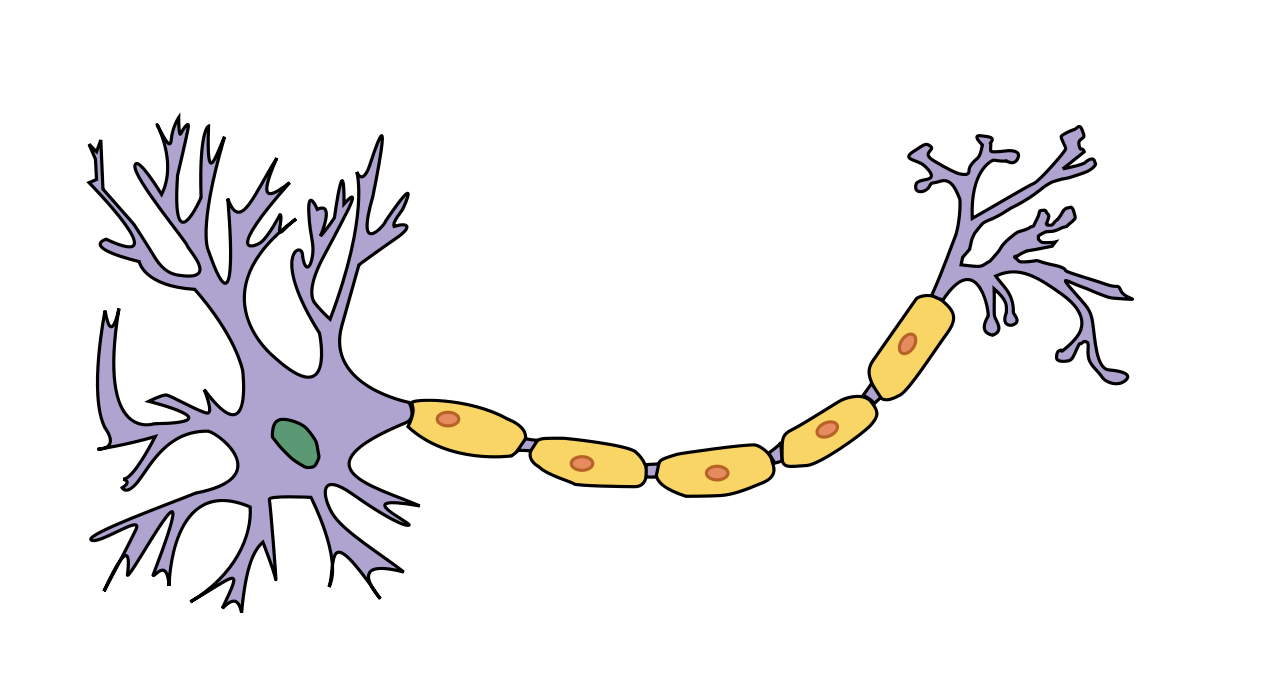
\includegraphics[width=\textwidth]{figures/figures/neuron.png}
  \end{center}
  \caption[A basic rendering of a biological neuron]{A basic rendering of a biological neuron.  Signals are received through the branching dendrites to the left of the image.  The cell body integrates and retransmits signals to other cells through the axon, which runs horizontally from left to right in the figure.  Biological nervous systems are based upon a repeated structure of neurons to carry signals over long distances.}

  \label{neuron}
\end{figure}


Artificial neural networks offer only a crude approximation of a true biological nervous system. 



Feedforward graph. \cite{reed1999neural}

Each node is connected to nodes in the previous layers.  

Node is represented by a vector of weights which determine response to input vector.  


Output is result of nonlinearity

Layer structure, or architecture, is arbitrary.  Multilayer networks are popular. 


Inputs can be anything.  Many cases involve input features which are engineered for a particular problem specification.  In the case of image processing, it is not uncommon to use all pixels from an image as the input layer.  

\begin{figure}[t]
  \begin{center}
    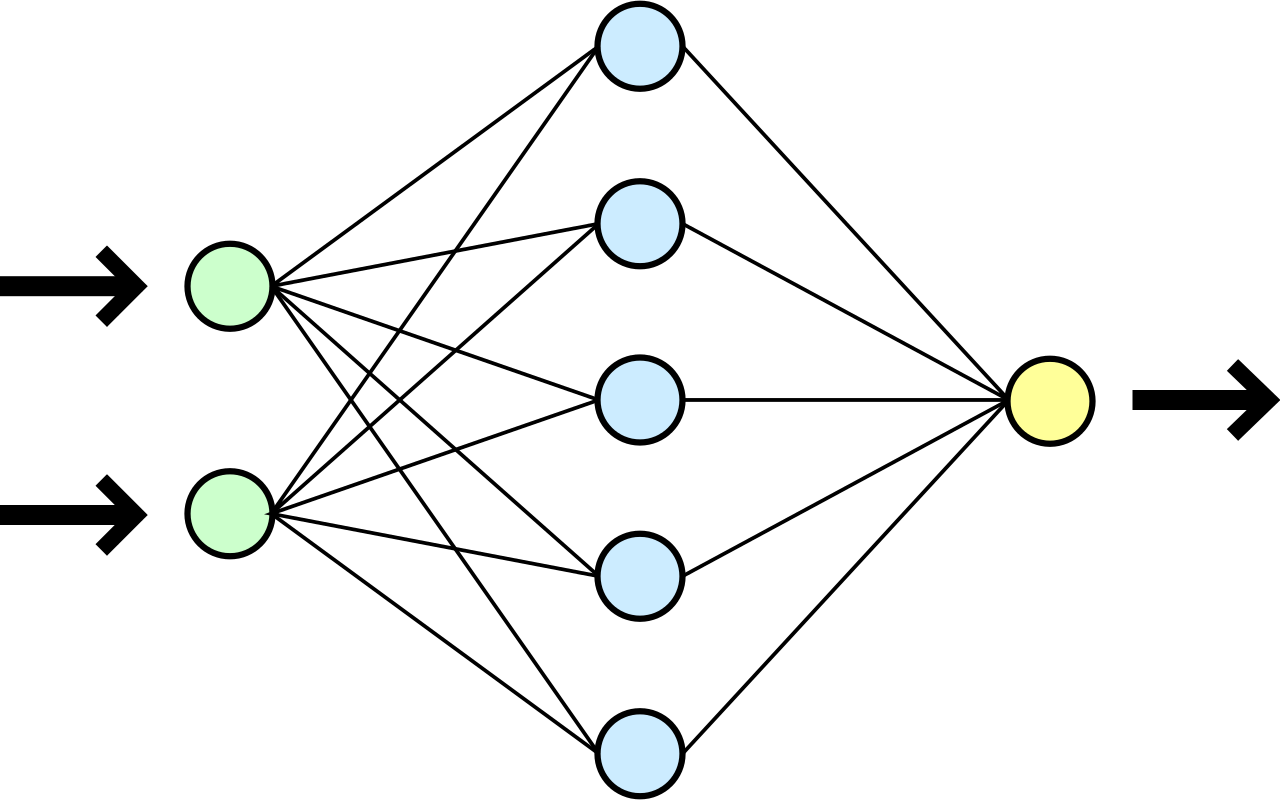
\includegraphics[width=0.6\textwidth]{figures/figures/basicNN.png}
  \end{center}
  \caption[Visualization of a simple neural network ]{Visualization of a simple neural network.  This network has an input layer (green) with two nodes, a hidden layer (blue) with five nodes, and an output layer (yellow) with one node.}

  \label{nnet}
\end{figure}


\section{Supervised Learning -- Backpropagation}


Minimize objective function 

Gradient in each layer is propagated through to previous layer through chain rule. 



\section{Neural Network Enhancements}

Convolution\cite{lecun1995comparison,lecun2010convolutional,krizhevsky2012imagenet} ... scan a filter... position independent... many filters of a particular size per layer... filters trained through backpropagation 


\begin{figure}[t]
  \begin{center}
    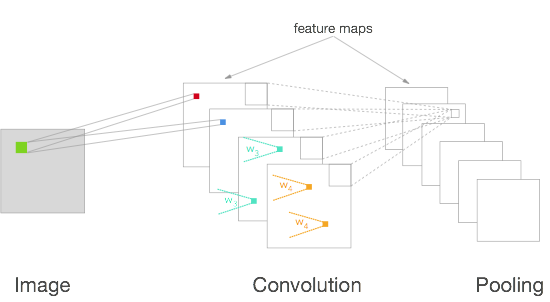
\includegraphics[width=0.6\textwidth]{figures/figures/convnet.png}
  \end{center}
  \caption[Example of a convolutional network ]{Example of a convolutional network.}

  \label{convnet}
\end{figure}



Pooling is used to reduce dimensionality. \cite{lecun2010convolutional} Image is downsampled by extracting a result from sub-regions of the image.  Two methods are commonly used, max pooling and average pooling.  Early results used non-overlapping pooling regions, although more recent efforts have seen good results from overlapping pooling regions \cite{krizhevsky2012imagenet}.  




Network-in-network\cite{lin2013network} .... inception module \cite{szegedy2014going}

Dropout... regularization technique. \cite{hinton2014dropout}



%%%%%%%%%%%%%%%%%%%%%%%%%%%%%%%%%%%%%%%%%%%%%%%%%%%%%%%%%%%%%%%%%%%%%%%%%%%%%%%%
